\documentclass[10pt]{article}
\usepackage[usenames]{color} %used for font color
\usepackage{amssymb} %maths
\usepackage{amsmath} %maths
\usepackage[utf8]{inputenc} %useful to type directly diacritic characters
\begin{document}
\begin{align*}\documentclass[a4paper,10pt]{article}
\usepackage{geometry}
\geometry{a4paper,left=30mm,top=35mm}
\usepackage[utf8]{inputenc}
\usepackage{amsmath}
\usepackage{graphicx}
\usepackage{listings}
\usepackage{color}
\graphicspath{ {images/} }
\usepackage{pgfplots}
\pgfplotsset{width=9cm,compat=1.9}

\definecolor{codegreen}{rgb}{0,0.6,0}
\definecolor{codegray}{rgb}{0.5,0.5,0.5}
\definecolor{codepurple}{rgb}{0.58,0,0.82}
\definecolor{backcolour}{rgb}{0.95,0.95,0.92}

\lstdefinestyle{mystyle}{
  backgroundcolor=\color{backcolour},   commentstyle=\color{codegreen},
  keywordstyle=\color{magenta},
  numberstyle=\tiny\color{codegray},
  stringstyle=\color{codepurple},
  basicstyle=\footnotesize,
  breakatwhitespace=false,         
  breaklines=true,                 
  captionpos=b,                    
  keepspaces=true,                 
  numbers=left,                    
  numbersep=5pt,                  
  showspaces=false,                
  showstringspaces=false,
  showtabs=false,                  
  tabsize=2
}
\lstset{style=mystyle}

\title{LWR Equation Simulation}
\author{Hongbei Chen, Xin Peng}

\begin{document}

\maketitle

\section{Model presentation}
\begin{center}
\begin{tikzpicture}
\begin{axis}[
    axis lines = left,
    xlabel = $Distance(x)$,
    ylabel = {$Density(\rho)$},
]

\addplot [
    domain=0:5000, 
    samples=100, 
    color=blue,
    ]
    {1.333*10^(-5)*x + 0.067};
\addlegendentry{$\rho(t=0)$}

\end{axis}
\end{tikzpicture}

\textbf{Figure 1:} The vehicle density road system, typically the initial state
\end{center}

Our system expresses the vehicle density(number of vehicles per meter) on a 5000-meter-long road. This quantity varies with space$(x)$ and time$(t)$, and we use $\rho(x,t)$ to denote it. In this case, we use the $Lighthill-Whitham-Richards(LWR)$ PDE to study the system. To observe the change of vehicle density on different spaces with time going by, we set the initial density(when t=0) of the road as shown in the Figure 1.\par
In order to quantify the evolution of the density of vehicles on the road, we use a mass balance for a small control volume of length $dx$ in the road. 
Following Figure 2, we have four terms in the balance:\par
1) $\rho(x,t)dx$ number of vehicles in the control volume $[x,x+dx]$ at $t$\par
2) $\rho(x,t+dt)dx$ number of vehicles in the control volume $[x,x+dx]$ at $t+dt$\par
3) $q(\rho(x,t))dt$ number of vehicles entering the control volume $[x,x+dx]$ between $t$ and $t+dt$ through $x$\par
4) $q(\rho(x+dx,t))dt$ number of vehicles entering the control volume $[x,x+dx]$ between $t$ and $t+dt$ through $x+dx$
\begin{center}
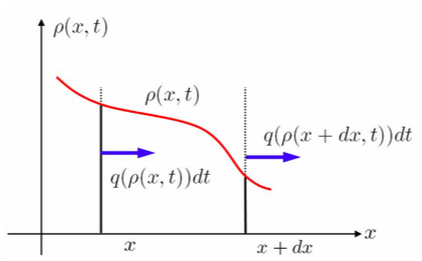
\includegraphics[scale=0.6]{fig2.png}\par
\textbf{Figure 2:} Illustration of the mass balance for the control volume $[x,x+dx]$
\end{center}
Equating the four terms in the balance, we obtain:\par
\begin{equation}\label{eq:1}
(\rho(x,t+dt)-\rho(x,t))dx = (q\rho(x,t))-q\rho(x+dx,t)))dt
\end{equation}
Dividing by $dt$ and $dx$, and taking the limit as $dt\rightarrow0$ and $dx\rightarrow0$, we obtain:\par
\begin{equation}\label{eq:2}
\frac{\partial \rho(x,t)}{\partial t}+\frac{\partial (q(\rho(x,t)))}{\partial x}=0
\end{equation}
This PDE can alternatively be rewritten as:\par
\begin{equation}\label{eq:3}
\frac{\partial \rho(x,t)}{\partial t}+q{}'(\rho(x,t))\frac{\partial (\rho(x,t))}{\partial x}=0
\end{equation}
\begin{center}
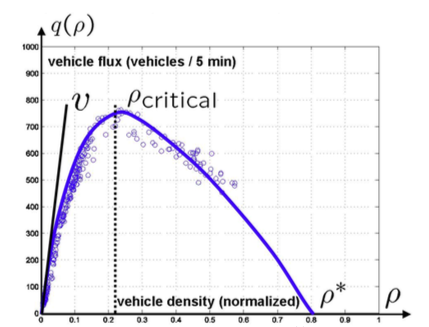
\includegraphics[scale=0.6]{fig3.png}\par
\textbf{Figure 3:} Greenshield model
\end{center}\par
$Greenshield$ $Model$ is an empirical measurement of the phenomenological law q with the density $\rho$ as shown in figure 3. Each of the dots is one measurement. The solid curve is a fit of the measurement. As can be seen, for small vehicle densities, the flux function increases almost linearly with the density (slope v). It reaches a maximum for a critical density, called $ \rho_{critical}$. For higher densities, it decreases until it finally reaches zero for a density $\rho^{*}$ called jam density.\par
According to figure 3, $Greenshield$ $flux$ $function$ is given by:
\begin{equation}\label{eq:4}
q(\rho)=v\rho(1-\frac{\rho}{\rho^{*}})
\end{equation}
where $\rho^{*}$ is the $jam$ $density$ and $v$ is the $free$ $flow$ $velocity$.\par
Combine equation (3) and (4), we get the final equation for our modeling:
\begin{equation}\label{eq:5}
\frac{\partial \rho(x,t)}{\partial t}+v(1-\frac{2\rho(x,t)}{\rho^{*}})\frac{\partial (\rho(x,t))}{\partial x}=0
\end{equation}

\vspace{5mm}
\section{Implementation}

\begin{lstlisting}[language=Python, caption=Python Code]
import numpy as np
import matplotlib.pyplot as plt
from mpl_toolkits.mplot3d import Axes3D

"""
Data structure creation and initialisation
"""
# Global parameters
T_final=3600 # time duration
N_t=500 # number of time steps: the time step value dt is computed later
X_final=5000 # road length
N_x=100 # number of space steps: the space step value dx is computed later
rho0=0.2 #jam density in Greenshield flux function(number of vehicles/m)
v0=15 #free flow velocity(m/s)

# structures for visualization and computation of time/space steps
T,dt=np.linspace(0,T_final,num=N_t,endpoint=True,retstep=True)
X,dx=np.linspace(0,X_final,num=N_x,endpoint=True,retstep=True)
#set the range and sample number of time(T)–[0,3600]seconds in every 7.2 seconds
#set the range and sample number of distance(X)–[0,5000]meters in every 50 meters
print("dx = ",dx,"  dt = ",dt)

# structure for simulation: density as a function of space and time
rho = np.zeros((N_x,N_t))
# initialization of the density at time 0 with a continuous function
for x in range(int(N_x/2)):
    rho[x][0] = rho0/3+rho0*x/N_x/3 # from rho0/3 to rho0/2
for x in range(int(N_x/2),N_x):
    # rho[x][0] = rho0/3+rho0*x/N_x/3 # from rho0/2 to rho0*2/3
    rho[x][0] = rho0/3+rho0*x/N_x/3
print("t = 0")
plt.plot(X,rho[:,0])
plt.show()#plot the density in the range of x at t=0

    
"""
Start the main simulation loop
Note that the naive Euler integration scheme is ALWAYS numerically unstable
Learn about Von Neumann stability analysis
And use the simple (stable) Lax scheme
But stability needs the Courant Friedrichs Levy condition to be verified
Trick: if unstable, decrease value of dt
"""
for t in range(N_t-1): # at timestep t, compute rho at t+1
    for x in range(1,N_x-1):
        #calculate density at t+1 on i based on density at t on i and i+1
        dr = v0*dt/dx*(2*rho[x][t]/rho0-1)*(rho[x+1][t]-rho[x-1][t])/2
        r = (rho[x-1][t]+rho[x+1][t])/2 + dr #this is Lax Scheme
        rho[x][t+1] = r
    # for x==N_x, we take the derivative backward
    x = 0
    dr = v0*dt/dx*(2*rho[x][t]/rho0-1)*(rho[x+1][t]-rho[x][t])
    r = (rho[x][t]+rho[x+1][t])/2 + dr
    rho[x][t+1] = r
    x = N_x-1
    dr = v0*dt/dx*(2*rho[x][t]/rho0-1)*(rho[x][t]-rho[x-1][t])
    r = (rho[x][t]+rho[x-1][t])/2 + dr
    rho[x][t+1] = r
    if((t+1)%int(N_t/5)==int(N_t/5)-1):
        print("t = ",t)
        plt.plot(X,rho[:,t])
        plt.show()#plot the density in the range of x at t=98,198,298,398,498
    
        
X,T = np.meshgrid(X,T)
Z = rho.reshape(X.shape)

fig=plt.figure()
ax=Axes3D(fig)
ax.plot_surface(X,T,Z, rstride=1, cstride=1, cmap='rainbow')
plt.show()#plot the 3d figure
\end{lstlisting}
The most important part to determine stability of the system lies in line 47 and 48 in the Listing 1. A stable system would have the same code in listing 1 which is:
\begin{lstlisting}[language=Python, caption=Stable Code]
dr = v0*dt/dx*(2*rho[x][t]/rho0-1)*(rho[x+1][t]-rho[x-1][t])/2
r = (rho[x-1][t]+rho[x+1][t])/2 + dr
\end{lstlisting}
Whereas an unstable system would have the below code to replace the stable one:
\begin{lstlisting}[language=Python, caption=Unstable Code]
 dr = v0*dt/dx*(2*rho[x][t]/rho0-1)*(rho[x+1][t]-rho[x][t])
 r = rho[x][t] + dr
\end{lstlisting}
\vspace{5mm}
\section{Results}
\includegraphics[scale=1]{plot.png}\par

\medskip
\end{document}
\end{align*}
\end{document}